


\chapter{Introduction}\label{ch:intro}


\begin{quote}
{\large ``L'intelligence est une adaptation.''\\
\cite{piaget:1966}}
\end{quote}


\noindent One of the hardest problems in artificial intelligence and robotics is what has been called the {\em symbol grounding problem} \citep{harnad:1990}. The question how ``seemingly meaningless symbols become meaningful" \citep{harnad:1990} is a question that also holds grip of many philosophers for already more than a century, e.g. \citep{bretano:1874,searle:1980,dennett:1991}\footnote{In philosophy the problem is usually addressed with the term {\em intentionality} introduced by \citep{bretano:1874}.}. With the rise of artificial intelligence (AI), the question has become very actual, especially within the symbolic paradigm \citep{newell:1990}\footnote{In the classical and symbolic AI the problem has also been addressed in what is known as the {\em frame problem} \citep{pylyshyn:1987}.}. The symbol grounding problem is still a very hard problem in AI and especially in robotics \citep{pfeiferscheier:1999}.

The problem is that an agent, be it a robot or a human, perceives the world in analogue signals. Yet humans have the ability to categorise the world in symbols that they, for instance may use for language. The perception of something, like e.g. the colour red, may vary a lot when observed under different circumstances. Nevertheless, humans are very good at recognising and naming this colour under these different conditions. For robots, however, this is extremely difficult. In many applications the robots try to recognise such perceptions based on the rules that are pre-programmed. But there are no singular rules that guide the conceptualisation of red. The same argument holds for many, if not all perceptions. A lot of solutions to the symbol grounding problem have been proposed, but there are still many limitations on these solutions. 

Intelligent systems or, as \citet{newell:1980} called them {\em physical symbol systems} should amongst others be able to use symbols, abstractions and language. These symbols, abstractions and language are always about something. But how do they become that way? There is something going on in the brains of language users that give meaning to these symbols. What is going on is not clear. It is clear from neuroscience that active neuronal pathways in the brain activate mental states. But how does this relate to objects and other things in the real world? According to \citet{maturanavarela:1992} there is a structural coupling between the things in the world and an organism's active pathways. \citet{wittgenstein:1958} stresses the importance of how language is used to make a relation with language and its meaning. The context of what he called a language game and the purpose of the language game establishes the meaning of it. According to these views, the meaning of symbols is established for a great deal by the interaction of an agent with its environment and is context dependent. A view that has been adopted in the field of pragmatics and situated cognition \citep{clancey:1997}.

In traditional AI and robotics the meaning of symbols was predefined by the programmer of the system. Besides that these systems have no knowledge about the meaning of these symbols, the symbols' meanings were very static and could not deal with different contexts or varying environments. Early computer programs that modelled natural language, notably SHRDLU \citep{winograd:1972} were completely pre-programmed, and hence could not handle the complete scope of a natural language. It could only handle that part of the language that was pre-programmed. SHRDLU has been programmed {\em as if} it were a robot with an eye and arm that was operating in a blocks world. Within certain constrictions, SHRDLU could manipulate English input such that it could plan particular goals. However, the symbols that SHRDLU was manipulating had no meaning for the virtual robot. Shakey, a real robot operating in a blocks world, did solve the grounding problem. But Shakey was limited to the knowledge that had been pre-programmed.

Later approaches to solve the grounding problem on real world multi-agent systems involving language have been investigated by \citet{yancostein} and \citet{billard:1997a}. In the work of Yanco and Stein the robots learned to communicate about actions. These actions, however, were pre-programmed and limited, and are therefore limited to the meanings that the robots had. In \citet{billard:1997a} one robot had pre-programmed meanings of actions, which were represented in a neural network architecture. A student robot had to learn couplings between communicated words and actions it did to follow the first robot. In this work the student robot learned to ground the meaning of its actions symbolically by associating behavioural activation with words. However, the language of the teacher robot was pre-programmed and hence the student could only learn what the teacher knows.

In the work of Billard and Hayes, the meaning is grounded in a situated experiment. So, a part of the meaning is situated in the context in which it is used. However, the learned representation of the meaning is developed through bodily experiences. This is conform the principle of {\em embodiment} \citep{lakoff:1987}, in which the meaning of something is represented according to bodily experiences. The meaning represented in someone's (or something's) brain depends on previous experiences of interactions with such meanings. The language that emerges is therefore dependent on the body of the system that experiences. This principle is made clear very elegantly by Thomas Nagel in his famous article {\em What's it like to be a bat?} \citep{nagel:1974}. In this article Nagel argues that it is impossible to understand what a bat is experiencing because it has a different body with different sensing capabilities (a bat uses echolocation to navigate). A bat approaching a wall must experience different meanings (if it has any) than humans would have when approaching a wall. Thus a robot that has a different body than humans will have different meanings. Moreover, different humans have different meaning representations because they encountered different experiences.

This book presents a series of experiments in which two robots try to solve the symbol grounding problem. The experiments are based on a recent approach in AI and the study of language origins, proposed by Luc \citet{steels:1996a}. In this new approach behaviour-based AI \citep{steelsbrooks:1993} is combined with new computational approaches to the language origins and multi-agent technology. The ideas of Steels have been implemented on real mobile robots so that they can develop a grounded lexicon about objects they can detect in their real world, as reported first in \citep{steelsvogt:1997}. This work differs from the work of \citep{yancostein,billard:1997a} in that no part of the lexicon and its meaning has been programmed. Hence their representation is not limited due to pre-programmed relations.

The next section introduces the symbol grounding problem in more detail. This section first discusses some theoretical background on the meaning of symbols after which some practical issues on symbol grounding are discussed. The experiments are carried out within a broader research on the origins of language, which is presented in \sectref{s:intro:origins}. A little background on human language acquisition is given in \sectref{s:intro:acquisition}. The research goals of this book are defined in \sectref{s:intro:goals}. The final section of this chapter presents the outline of this book.

\section{Symbol Grounding Problem}

\subsection{Language of Thought}

Already for more than a century philosophers ask themselves how is it possible that we seem to think in terms of symbols which are {\em about} something that is in the real world. So, if one manipulates symbols as a mental process, one could ask what is the symbol (manipulation) about? Most explanations in the literature are however in terms of symbols that again are about something as in folk-psychology intentionality is often explained in terms of beliefs, desires etc. For instance, according to Jerry \citet{fodor:1975} every concept is a propositional attitude. Fodor hypothesises a {\em Language of Thought} to explain why humans tend to think in a {\em mental} language rather than in natural language alone.

Fodor argues that concepts can be described by symbols that represent {\em propositions} towards which attitudes (like {\em beliefs}, {\em desires}) can be attributed. Fodor calls these symbols {\em propositional attitudes}. If $P$ is a proposition, then the phrase ``I belief that $P$'' is a propositional attitude. According to Fodor, all mental states can be described as propositional attitudes, so a mental state is a belief or desire {\em about} something. This {\em something}, however is a proposition, which according to Fodor is {\em in the head}. But mental states should be about something that is in the real world. That is the essence of the symbol grounding problem. The propositions are symbol structures that are represented in the brain, sometimes called {\em mental representations}. In addition, the brain consists of rules that describe how these representations can be manipulated. The language of thought, according to Fodor, is constituted by symbols which can be manipulated by applying existing rules. Fodor further argues that the language of thought is innate, and thus resembles Chomsky's universal grammar very well.

Concepts are in this Computational Theory of Mind (as Fodor's theory sometimes is called) constructed from a set of propositions. The language of thought (and with that concepts) can, however, not be learned according to Fodor, who denies:

\index{Fodor, Jerry}
\index{language!of thought}

\begin{quote}
[r]oughly, that one can learn a language whose expressive power is greater than that of a language that one already knows. Less roughly, that one can learn a language whose predicates express extensions not expressible by those of a previously available representational system. Still less roughly, that one can learn a language whose predicates express extensions not expressible by predicates of the representational system {\em whose employment mediates the learning}. \cite[p. 86, Fodor's italics]{fodor:1975}
\end{quote}


According to this, the process of concept learning is the testing of hypotheses that are already available at birth.

Likewise Fodor argues that perception is again the formulating and testing of hypotheses, which are already available to the agent.


So, Fodor argues that, since one cannot learn a concept if one does not have the conceptual building blocks of this concept. And since perception needs such building blocks as well, concept learning does not exist and therefore concepts must be innate. This is a remarkable finding, since it roughly implies that all that we know is actual innate knowledge. Fodor called this innate inner language ``Mentalese''. It must be clear that it is impossible to have such a language. As Patricia S. Churchland puts it:

\begin{quote}
[The Mentalese hypothesis] entails the ostensibly new concepts evolving in the course of scientific innovation - concepts such as atom, force field, quark, electrical charge, and gene - are lying ready-made in the language of thought, even of a prehistoric hunter-gatherer... The concepts of modern science are defined in terms of the theories that embed them, not in terms of a set of ``primitive conceptual atoms,'' whatever those may be. \cite[p. 389]{p.s.churchland:1986}
\end{quote}


Although the Computational Theory of Mind is controversial, there are still many scientist who adheres to this theory and not the least many AI researchers. This is not surprising, since the theory tries to model cognition computationally, which of course is a nice property since computers are computational devices. It will be shown however that Fodor's Computational Theory of Mind is not necessary for concept and language learning. In particular it will be shown that robots can be developed that can acquire, use and manipulate symbols which are about something that exists in the real world, {\em and} which are initially not available to the robots.
	
\subsection{Understanding Chinese}


\bigskip\noindent
\index{Chinese Room|(}
\index{Searle, John|(}
This so-called symbol grounding problem was made clear excellently by John R. Searle with a gedanken experiment called the {\em Chinese Room} \citep{searle:1980}. In this experiment, Searle considers himself standing in a room in which there is a large data bank of Chinese symbols and a set of rules how to manipulate these symbols. Searle, while in the room receives symbols that represent a Chinese expression. Searle, who does not know any Chinese, manipulates these symbols according to the rules such that he can output (other) Chinese symbols as if it was responding correctly in a human like way, but only in Chinese. Moreover, this room passes the Turing test for speaking and understanding Chinese.

Searle claims that this room cannot understand Chinese because he himself does not. Therefore it is impossible to build a computer program that can have mental states and thus being what Searle calls a {\em strong AI}\footnote{It is not the purpose of this book to show that computer programs can have mental states, but to show that symbols in a robot can be about something.}. It is because Searle inside the room does not know what the Chinese symbols are about that Searle concludes that the room does not understand Chinese. Searle argues with a logical structure by using some of the following premises \cite[p. 39]{searle:1984}:

\begin{enumerate}
\item Brains cause minds.
\item Syntax is not sufficient for semantics.
\item Computer programs are entirely defined by their formal, or syntactical, structure.
\item Minds have mental contents; specifically, they have semantic contents.
\end{enumerate}

Searle draws his conclusions from these premises in a correct logical deduction, but for instance premise (1) seems incomplete. This premise is drawn from Searle's observation that:

\begin{quote}
(A)ll mental phenomena ... are caused by processes going on in the brain. \cite[p. 18]{searle:1984}.
\end{quote}

One could argue in favour of this, but Searle does not mention what causes these brain processes. Besides metabolic and other biological processes that are ongoing in the brain, brain processes are caused by sensory stimulation and maybe even by {\em sensorimotor} activity as a whole. So, at least some mental phenomena are to some extent caused by an agent's\footnote{I refer to an agent when I am talking about an autonomous agent in general, be it a human, animal, robot or something else.} interaction with its environment.

Premise (3) states that computer programs are entirely defined by their formal structure, which is correct. Only Searle equates formal with syntactical, which is correct when syntactic means something like {\em manipulating symbols according to the rules of the structure}. The appearance of {\em symbols} in this definition is crucial, since they are by definition about something. If the symbols in computer programs are about something, the programs are also defined by their semantic structure.

Although Searle does not discuss this, it may be well possible that he makes another big mistake in assuming that he (the central processing unit) is the part where all mental phenomena should come together. An assumption which is debatable \citep[see, e.g., ][]{dennett:1991,edelman:1992}. It is more likely that consciousness is more distributed. But it is not the purpose here to explain consciousness, instead the question is how are symbols about the world. The Chinese Room is presented to make clear what the problem is and how philosophers deal with it.

Obviously Searle's Chinese Room argument found a lot of opposition in the cognitive science community. The critique presented here is in line with what has been called the {\em system's reply} and to a certain extend the {\em robot's reply}\footnote{See for instance the critiques that appeared in the open peer commentary of Searle's 1980 article in the Behavioural and Brain Sciences.}. The system's reply holds that it is not the system who does not understand Chinese, but it is {\em Searle} who does not. The system as a whole does, since it passed the Turing test. 

The robot's reply goes as follows: The Chinese Room as a system does not have any other input than the Chinese symbols. So the system is a very unlikely cognitive agent. Humans have perceptual systems that receive much more information than only linguistic information. Humans perceive visual, tactile, auditory, olfactory and many other information; the Chinese Room does, as it seems, not. So, what if we build a device that has such sensors and like humans has motor capacities? Could such a system with Searle inside understand Chinese?

According to Searle in his answer to both the system's as robot's reply \citep{searle:1984}, his argument still holds. He argues that both the system's reply and the robot's reply do not solve the syntax vs. semantics argument (premise (2)). But the mistake that Searle makes is that premise (3) does not hold, thus making premise (2) redundant. Furthermore, in relation to the robot's reply Searle fails to notice the fact that brain processes are (partly) caused by sensory input and thus mental phenomena are indirectly caused by sensory stimulation.

And even if Searle's arguments are right, in his answer to the robot's reply he fails to understand that a robot is actually a {\em machine}. It is not just a computer that runs a computer program. And as Searle keeps on stressing:

\begin{quote}
'Could a machine think?' Well, in one sense, of course, we are all machines. (...) [In the] sense in which a machine is just {\em a physical system which is capable of performing certain kinds of operations} in that sense we are all machines, and we can think. So, trivially there are machines that can think. \cite[p. 35, my italics]{searle:1984}
\end{quote}

The reason why the phrase ``a physical system which is capable of performing certain kinds of operations'' is emphasised is because it is exactly that what a robot is. A robot is more than a computer that runs a computer program.

A last point that is made in this section is that Searle does not speak about development. Could Searle learn to understand Chinese if it was in the room from its birth and that he learned to interpret and manipulate the symbols that were presented to him? It is strange that a distinguished philosopher like Searle does not understand that it is possible to develop computer programs which can learn.

\bigskip\noindent
\index{Chinese Room|)}
\index{Searle, John|)}
The Chinese Room introduced the symbol grounding problem as a thought experiment that inspired Stevan Harnad to define his version of the problem \citep{harnad:1990}. Although controversial, the Chinese Room experiment showed that there are nontrivial problems arising when one builds a cognitive robot that should be able to acquire a meaningful language system. The arguments presented against the Chinese Room are the core of the argument why robots can ground language. As shall become clear, there's more to language than just symbol manipulation according to some rules.

\subsection{Symbol Grounding: Philosophical or Technical?}

\label{s:intro:semiotic}

\index{symbol grounding problem|(}
Although it might seem very philosophical up to now, this book in no way tries to solve the philosophical problem of what is meaning. In fact there is no attempt being made in solving any philosophical problem. The only thing that is done here is to translate a philosophical problem into a technical problem, which will be tackled in this work. The solution to the technical problem could then be the meat for the philosophers to solve their problem.


Before discussing the symbol grounding problem in more technical detail, it is useful to come up with a working definition of what is meant with a symbol. Harnad's definition of a symbol is very much in line with the standard definition used in artificial intelligence. This definition is primarily based on {\em physical symbol systems} introduced by Newell and Simon \citep{newell:1980,newell:1990}. According to Harnad symbols are basically a set of arbitrary tokens that can be manipulated by rules made of tokens; the tokens (either atomic or composite) are ``semantically interpretable'' \citep{harnad:1990}.

\index{semiotics|(}
\index{symbol|(}
\index{sign|see{symbol}}
\index{Peirce, C.S.|(}

In this book a definition taken from semiotics will be adopted. Following Charles Sanders Peirce and Umberto Eco \citep{eco:1976,eco:1986} a symbol will be equalled with a {\em sign}. Using a different, but more familiar terminology than Peirce  \citep{noth:1990}, a sign consists of three elements \citep{chandler:1994}\footnote{An instructive introduction into the theory of semiotics can be found on the world-wide web \citep{chandler:1994}. The work of Peirce is collected in \citep{peirce:1931}.}:

\begin{description}
\item[Representamen] The form which the sign takes (not necessarily material).
\item[Interpretant] The sense made of the sign.
\item[Object] To which the sign refers. 
\end{description}

\index{form}
\index{meaning}
\index{referent}


Rather than using Peirce's terms, the terms adopted in this book are {\em form} for representamen, {\em meaning} for interpretant and {\em referent} for object. The adopted terminology is in line with Steels' terminology \citep{steels:2000}. It is also interesting to note that the Peircean sign is not the same as the Saussurean sign \citep{saussure:1974}. De Saussure does not discuss the notion of the referent. In de Saussure's terminology the form is called {\em signifier} and the meaning is called the {\em signified}.

\index{Saussure, Ferdinand de}

\begin{figure}
\centerline{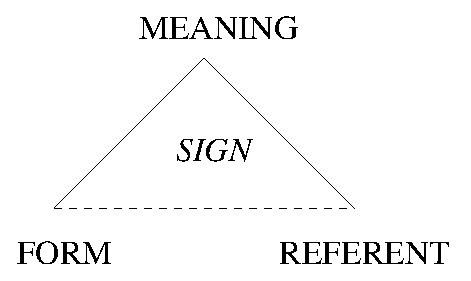
\includegraphics[width=6.6cm]{introduction/semiotic3.eps}}
\caption{A semiotic triangle shows how a referent, meaning and form are related as a sign.}
\label{f:intro:semiotic}
\end{figure}

How the three units of the sign are combined is often illustrated with the semiotic triangle (\figref{f:intro:semiotic}). According to Peirce, a sign becomes a {\em symbol} when its form, in relation to its meaning ``is arbitrary or purely conventional - so that the relationship must be learnt'' \citep{chandler:1994}. The relation can be conventionalised in language. According to the semiotic triangle and the above, a symbol is {\em per definition} grounded.

In the experiments reported in this book, the robots try to develop a shared and grounded lexicon about the real world objects they can detect. They do so by communicating a name of the categorisation of a real world object. In line with the theory of semiotics, the following definitions are made:

\begin{description}

\item[Referent] The referent is the real world object that is subject of the communication.\index{referent}

\item[Meaning] The meaning is the categorisation that is made of the real world object and that is used in the communication.\index{meaning}

\item[Form] The form is the name that is communicated. In principle its shape is arbitrary, but in a shared lexicon it is conventionalised through language use.\index{form}

\item[Symbol] A symbol is the relation between the referent, the meaning and the form as illustrated in the semiotic triangle.\index{symbol}

\end{description}


\index{semiotics|)}
\index{symbol|)}
\index{Peirce, C.S.|)}


This brings us to the technically hard part of the symbol grounding problem that remains to be solved: How can an agent construct the relations between a form, meaning and referent? In his article \citet{harnad:1990} recognises three main tasks of grounding symbols:

\begin{enumerate}
\index{symbol grounding problem!iconisation}
\item {\bf Iconisation}\footnote{The terms icon and iconisation as they are used by Harnad, which will be adopted here, should not be confused with Peirce's notion of these terms.} Analogue signals need to be transformed to {\em iconic representation} (or icons).
\index{symbol grounding problem!discrimination}
\item {\bf Discrimination} ``[The ability] to judge whether two inputs are the same or different, and, if different, how different they are.'' Note that in Harnad's article, discrimination is already pursued at the perceptual level. In this book, discrimination is done at the categorical level.
\index{symbol grounding problem!identification}\index{invariance}
\item {\bf Identification} ``[The ability] to be able to assign a unique (usually arbitrary) response -- a `name' -- to a class of inputs, treating them all as equivalent or {\em invariant} in some respect.'' \cite[my italics]{harnad:1990}
\end{enumerate}


So, what is the problem? Analogue signals can be iconised (or recorded) rather simple with meaningless sub-symbolic structures. The ability to discriminate is easy to implement just by comparing two different sensory inputs. The ability to identify requires to find {\em invariant} properties of objects, events and state of affairs. Since finding distinctions is rather easy, the big problem in grounding actually reduces to identifying

\begin{quote}
invariant features of the sensory projection that will reliably distinguish a member of  a category from any non-members with which it could be confused. \citep{harnad:1990}
\end{quote}

Although people might disagree, for the roboticists this is not more than a technical problem. The question is whether or not there exist real invariant features of a category in the world. This probably could be doubted quite seriously \citep[see, e.g., ][]{harnad:1993}. For the time being it is assumed that there are invariant properties in the world and it will be shown that these {\em invariants} can be found if an embodied agent is equipped with the right physical body and control. The latter inference is in line with the {\em physical grounding hypothesis} \citep{brooks:1990}, which will be discussed below.

 Stevan Harnad proposes that the SGP for a robot could possibly be solved by invoking (hybrid) connectionist models with a serious interface to the outside world in the form of {\em transducers} (or sensors) \citep{harnad:1993}. Harnad, however admits that the symbol grounding problem also might be solved with other than connectionist architectures.

\subsection{Grounding Symbols in Language}

In line with the work of Luc Steels the symbols are grounded in language, see e.g. \citep{steels:1997a,steels:2000}. Why grounding symbols in language directly and not ground the symbols first and develop a shared lexicon afterwards? Associating the grounded symbols with a lexicon is then a simple task, see e.g. \citep{oliphant:1997,steels:1996a}. However, as \citet{wittgenstein:1958} pointed out, the meaning of something depends on how it is used in language. It is situated in the environment of an agent and depends on the bodily experience of it. Language use gives feedback on the appropriateness of the sense that is made of a referent. So, language gives rise to the construction of meanings and the construction of meaning gives rise to language development. Hence, meaning co-evolves with language.\index{language!game}\index{co-evolution}

That this approach seems natural can be illustrated with Roussau's paradox. Although for communication categorisation of reality needs to be similar to different language users, different languages do not always employ the same categorisations. For instance, there are different referential frames to categorise spatial relations in different language communities. In English there are spatial relations like {\em left}, {\em right}, {\em front} and {\em back} relative to some axis. However in Tzetal, a Mayan language, this frame of reference is not used not used. The Tzetal speakers live in an area with mountains and their frame of reference is absolute in relation to the mountain they are on. The spatial relations in this language can be translated with {\em uphill}, {\em downhill} and {\em across}. If something is higher up the mountain in relation to the speaker, they can say 'this something is uphill of me'.

So, if a novel language user enters a language society, how would it know how to categorise such a spatial relation? To know this, the new language user has to learn how to categorise the reality in relation to the language that is used by the particular language society. Therefore it is thought to be necessary to ground meaning in language. How lexicon development interacts with the development of meaning will become clearer in the remainder of this book.


\index{symbol grounding problem|)}
\index{physical!grounding hypothesis|(}
\subsection{Physical Grounding Hypothesis}\label{s:theory:pgh}

Another approach to grounding is physical grounding. In his article {\em Elephants Don't Play Chess} Rodney Brooks (1990) proposed the physical grounding hypothesis as an additional constraint to the physical symbol system hypothesis. 

\index{physical!symbol system}
\index{Brooks, Rodney|(}

\begin{quote}
The physical grounding hypothesis states that to build a system that is intelligent it is necessary to have its representations grounded in the physical world. \citep{brooks:1990}
\end{quote}

The advantage of the physical grounding hypothesis over physical symbol system hypothesis is that the system (or agent) is directly coupled to the real world through its set of sensors and actuators. 

\begin{quote}
Typed input and output are no longer of interest. They are not physically grounded. \citep{brooks:1990}
\end{quote}

In Brooks' approach symbols are not a necessary condition for intelligent behaviour anymore \citep{brooks:1990,brooks:1991}. Intelligent behaviour can emerge from a set of simple couplings of an agent's sensors with its actuators\footnote{Note that Brooks' approach does not necessarily invoke connectionist models.}, as is also shown in e.g. \citep{steelsbrooks:1993,steels:1994,steels:1996c}. An example is {\em wall following}. Suppose a robot has two simple behaviours: (1) the tendency to move towards the wall and (2) the tendency to move away from the wall. If the robot incorporates both behaviours at once, then the resulting {\em emergent} behaviour is wall following. Note that agents designed from this perspective have no cognitive abilities. They are reactive agents, like e.g. ants are, rather than cognitive agents that can manipulate symbolic meanings.

The argument that Brooks uses to propose the physical grounding hypothesis is that

\begin{quote}
[evolution] suggests that problem solving behaviour, language, expert knowledge and application, and reason, are all rather simple once the essence of being and reacting are available. That essence is the ability to move around in a dynamic environment, sensing the surroundings to a degree sufficient to achieve the necessary maintenance of life and reproduction. \citep{brooks:1990}
\end{quote}

\begin{figure}
\centerline{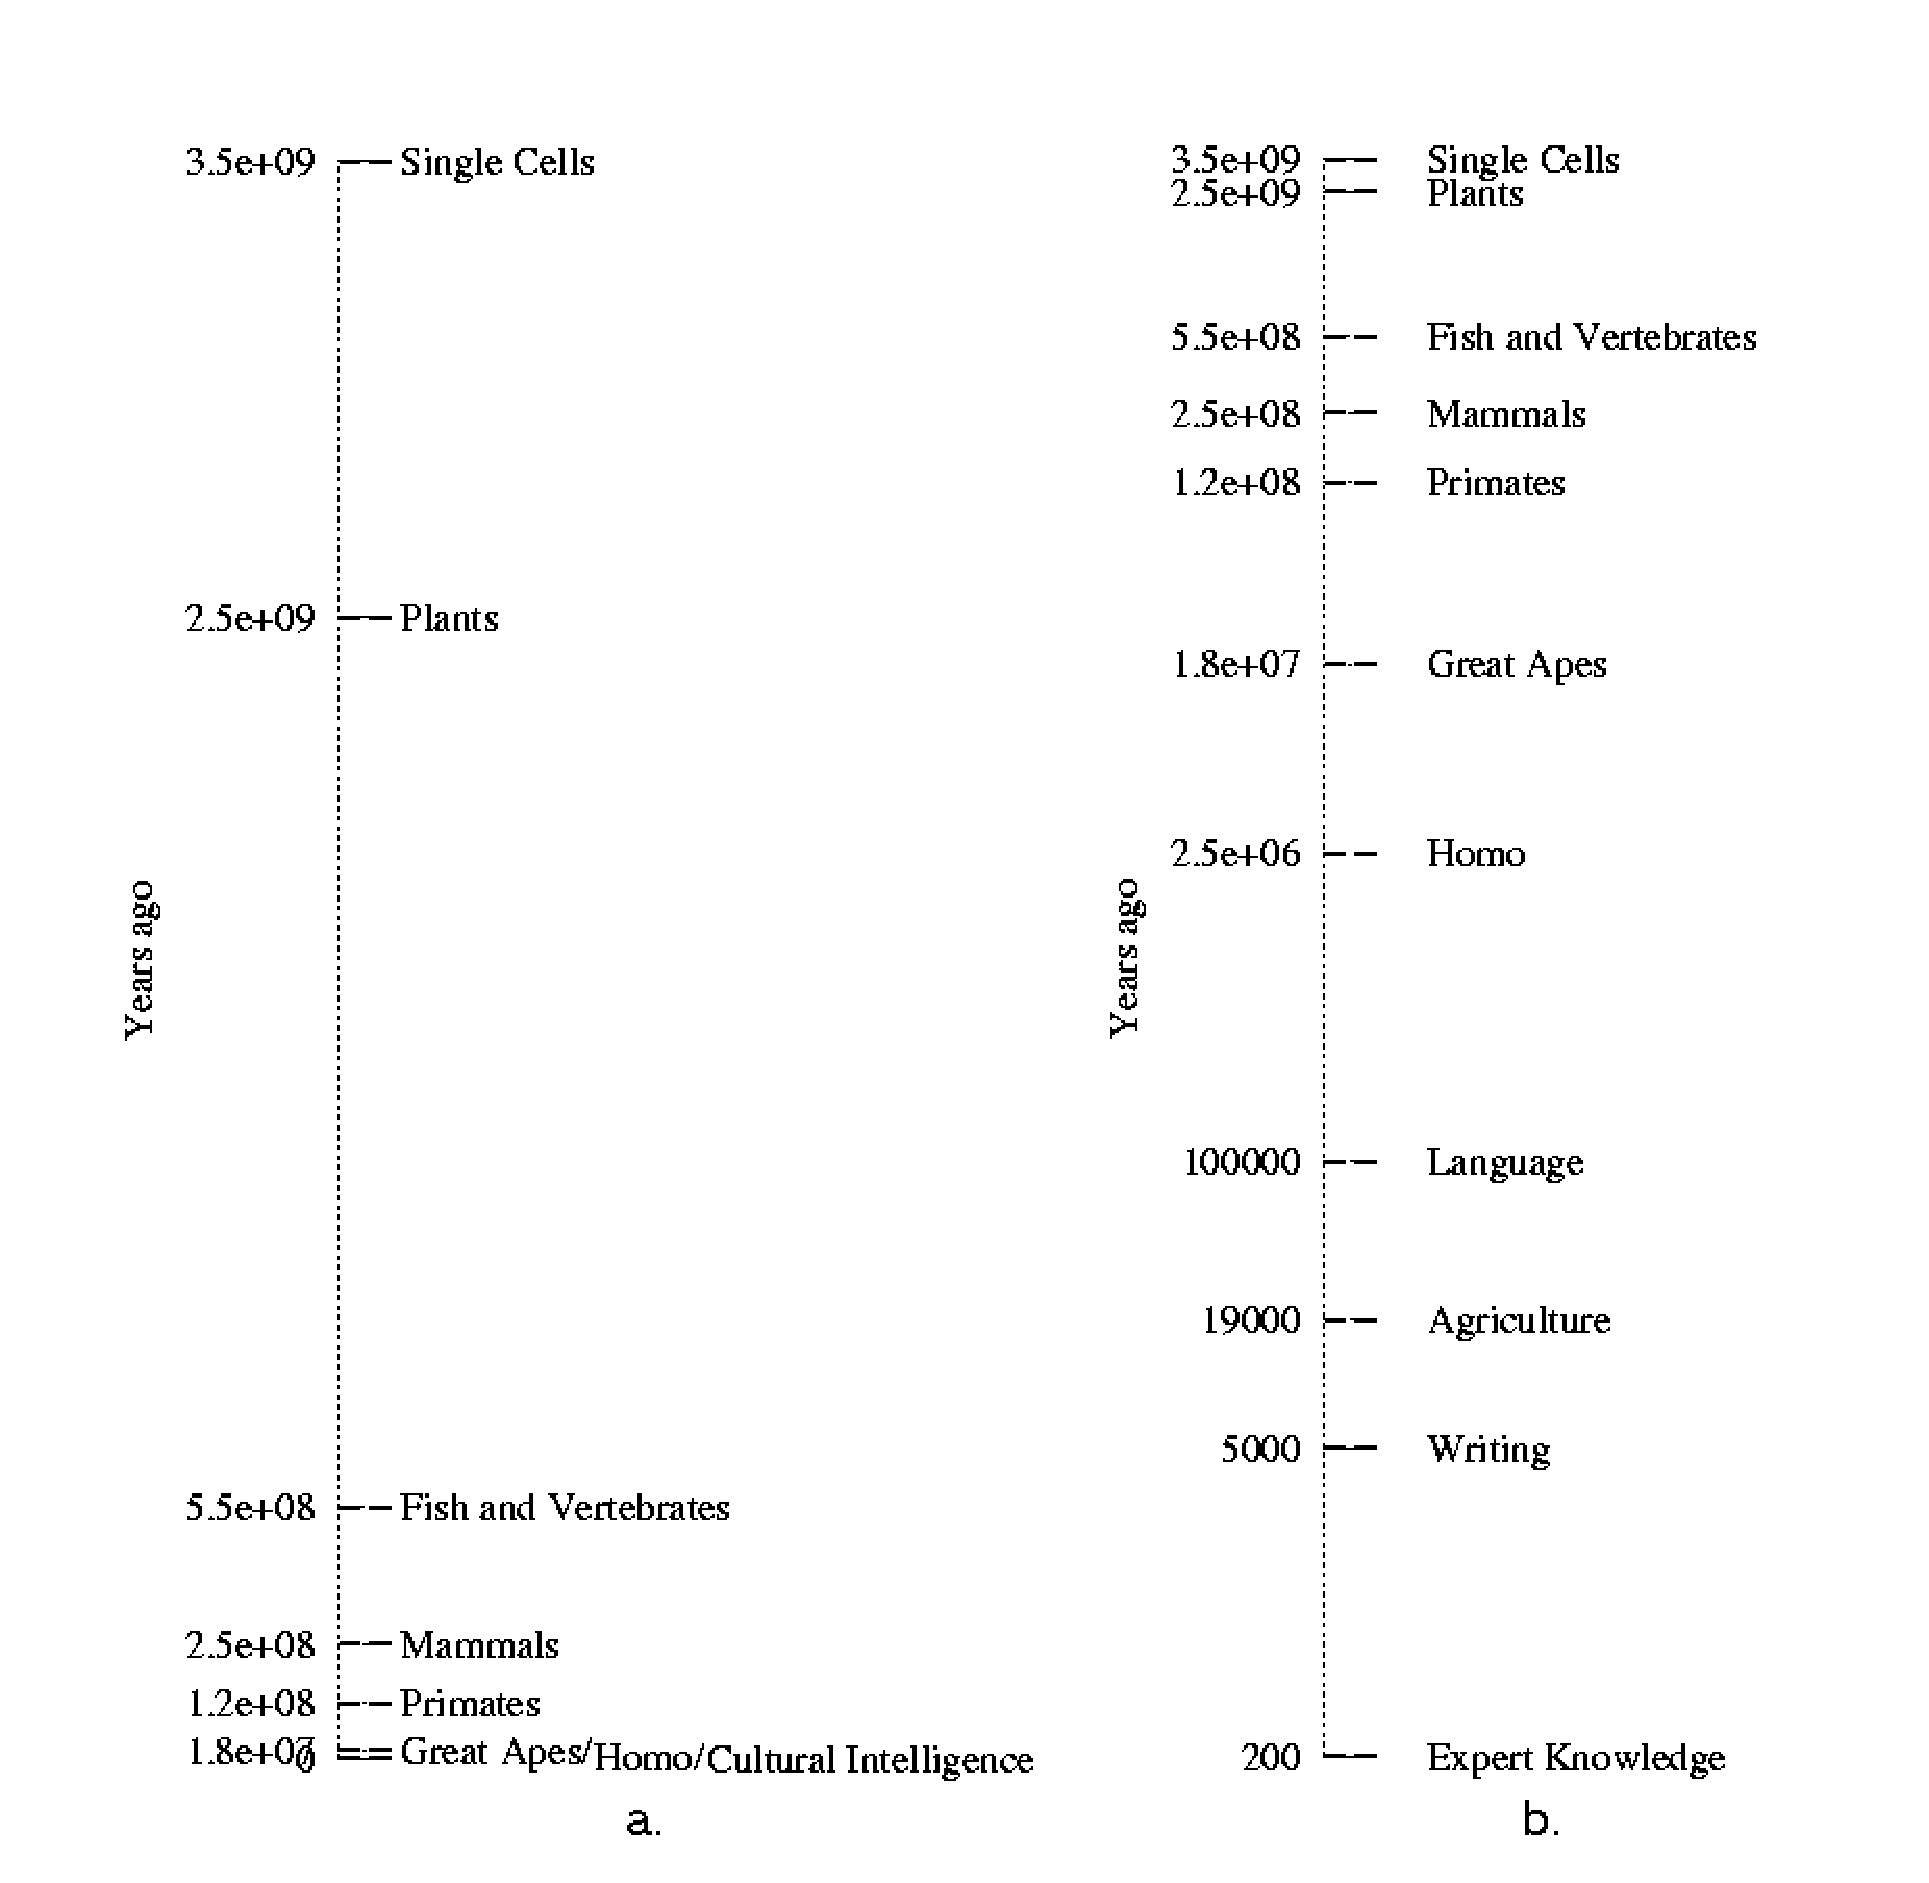
\includegraphics[width=12cm]{theory/evol.eps}}
\caption{\index{cultural evolution}(a) The evolutionary time-scale of life and cognitive abilities on earth. After the entrance of the Great Apes, evolution of man went so fast, that it cannot be shown on the same plot, unless it is shown in logarithmic scale, see (b). It appears from the plot that cultural evolution works much faster than biological evolution. Time-scale is adapted from (Brooks 1990).}
\label{f:theory:evolution}
\end{figure}


This rapid evolution is illustrated in \figref{f:theory:evolution}. Brooks also uses this argument of the rapid evolution of human intelligence as opposed to the slow evolution of life on earth in relation to symbols.

\begin{quote}
[O]nce evolution had symbols and representations things started moving rather quickly. Thus symbols are the key invention ... Without a carefully built physical grounding any symbolic representation will be mismatched to its sensors and actuators. \citep{brooks:1990}
\end{quote}

\index{physical!grounding hypothesis|)}
\index{Brooks, Rodney|)}
\index{subsumption architecture}
\index{situated embodiment}

To explore the physical grounding hypothesis, Brooks and his co-workers at the MIT AI Lab developed a software architecture called the {\em subsumption architecture} \citep{brooks:1986}. This architecture is designed to connect a robot's sensors to its actuators so that it {\em embeds the robot correctly in the world} \citep{brooks:1990}.  The point made by Brooks is that intelligence can emerge from an agent's physical interactions with the world. So, the robot that needs to be built should be both {\em embodied} and {\em situated}. The approach proposed by Brooks is also known as {\em behaviour-based} AI.


\subsection{Physical Symbol Grounding}
\index{physical!symbol grounding problem|(}
\index{physical!grounding hypothesis}
\index{symbol grounding problem}
\index{physical!symbol system}

The physical grounding hypothesis \citep{brooks:1990} states that intelligent agents should be grounded in the real world. However, it also states that the intelligence need not to be represented with symbols. According to the physical symbol system hypothesis the thus physically grounded agents are no cognitive agents. The physical symbol system hypothesis \citep{newell:1980} states that cognitive agents are {\em physical symbol systems} that have a \cite[p. 77]{newell:1990}

\begin{quote}
\begin{description}
\item[Memory]
Contains structures that contain symbol tokens\\
Independently modifiable at some grain size

\item[Symbols]
Patterns that provide access to distal structures\\
A symbol token is the occurrence of a pattern in a structure

\item[Operations]
Processes that take symbol structures as input and produce symbol structures as output

\item[Interpretation]
Processes that take symbol structures as input and execute operations

\item[Capacities]
Sufficient memory and symbols\\
Complete compositionality\\
Complete interpretability
\end{description}
\end{quote}


Clearly, an agent that uses language is a physical symbol system. It should have a memory to store an ontology and lexicon. It has symbols. The agent makes operations on the symbols and interprets them. Furthermore, it should have the capacity to do so. In this sense, the robots of this book are physical symbol systems.

A physical symbol system somehow has to represent the symbols. Hence the physical grounding hypothesis is not the best candidate. But since the definition of a symbol adopted in this book has an explicit relation to the referent, the complete symbol cannot be represented inside a robot. The only parts of the symbols that can be represented are the meaning and the form. Like in the physical grounding hypothesis, a part of the agent's knowledge is in the world. The problem is how the robot can {\em ground} the relation between internal representations and the referent? Although \citet{newell:1990} recognises the problem, he does not investigate a solution to it.

This problem is what \citep{harnad:1990} called the symbol grounding problem. Because there is a strong relation between the physical grounding hypothesis (that the robot has its knowledge grounded in the real world) and the physical symbol system hypothesis (that cognitive agents are physical symbol systems) it is useful to rename the symbol grounding problem in the {\em physical symbol grounding problem}.

The physical symbol grounding problem is very much related to the {\em frame problem} \citep{pylyshyn:1987}. The frame problem deals with the question how a robot can represent things of the dynamically changing real world and operate in it. In order to do so, the robot needs to solve the symbol grounding problem. 


As mentioned, this is a very hard problem. Why is the physical symbol grounding problem so hard? When sensing something in the real world under different circumstances, the physical sensing of this something is different as well. Humans are nevertheless very good at identifying this something under these different circumstances. For robots this is different. The one-to-many mappings of this something unto the different perceptions needs to be interpreted so that there is a more or less one-to-one mapping between this something and a symbol, i.e. the identification needs to be invariant. Studies have shown that this is an extremely difficult task for robots.

Already numerous systems have been physically grounded, see e.g. \citep{brooks:1990,steels:1994,barnesetal:1997,KroBunVlaMot99,taninolfi:1998,berthouzekuniyoshi:1998,pfeiferscheier:1999,billard:1997a,rosenstein:1998a,yancostein} and many more. However, a lot of these systems do not ground symbolic structures because they have no form (or arbitrary label) attached. These applications ground `simple' physical behaviours in the Brooksean sense. Only a few physically grounded systems mentioned above grounded symbolic structures. This is for instance in the case of \citep{yancostein,billard:1997a,rosenstein:1998a}. 


\citet{yancostein} developed a troupe of two robots that could learn to associate certain actions with a pre-defined set of words. One robot would decide what action is to be taken and communicates a relating signal to the other robot. The learning strategy they used was reinforcement learning where the feedback in their task completion was provided by a human instructor. If both robots performed the same task, a positive reinforcement was give, and when both robots did not, the feedback consisted of a negative reinforcement.

The research was primarily focussed on the learning of associations between word and meaning on physical robots. No real solution was attempted to solve the grounding problem and only a limited set of word-meaning associations were pre-defined. In addition, the robots learned by means of supervised learning with a human instructor. \citet{yancostein} showed however, that a group of robots could converge in learning such a communication system.


In \citet{billard:1997a} two robots grounded a language by means of imitation. The experiments consisted of a teacher robot, which had a pre-defined communication system, and a student robot, which had to learn the teacher's language by following it. The learning mechanism was provided by an associative neural network architecture called DRAMA. This neural network learned associations between communication signals and sensorimotor couplings. Feedback was provided by the student's evaluation if it was still following the teacher.

So, the language was grounded by the student using this neural network architecture, which is derived from Wilshaw networks. Associations for the teacher robot were pre-defined in their couplings and weights. The student could learn a limited amount of associations of actions and perceptions very rapidly \citep{billard:1998}.


\citet{rosenstein:1998a} developed a robot that could ground time series by using the so-called method of delays, which is drawn from the theory of non-linear dynamics. The time series that the robots produce by interacting in their environment are categorised by comparing their delay vectors, which is a low-dimensional reconstruction of the original time series, with a set of prototypes. The concepts the robots thus ground could be used for grounding word-meanings \citep{rosenstein:1998b}.

The method proposed by \citet{rosenstein:1998a} has been incorporated in a language experiment where two robots play follow me games to construct an ontology and lexicon to communicate their actions \citep{vogt:1999a,vogt:2000}. This was a preliminary experiment, but the results appear to be promising.

A similar experiment on language acquisition on mobile robots has been done by the same group of Rosenstein and Cohen at the University of Massachusetts \citep{oatesetal:1999}. The time series of a robot's actions are categorised using a clustering method for distinctions \citep{oates:1999}. Similarities between observed time series and prototypes are calculated using dynamical time warping. The thus conceptualised time series are then analysed in terms of human linguistic interactions, who describe what they see when watching a movie of the robot operating \citep{oatesetal:1999}.


Other research propose simulated solutions to the symbol grounding problem, notably \citep{cangelosiparisi:1998,cangelosi:1998}. In his work Angelo Cangelosi created an ecology of edible and non-edible mushrooms. Agents that are provided with neural networks learn to categorise the mushrooms from `visible' features into the categories of edible and non-edible mushrooms.

A problem with simulations of grounding is that the problem cannot be solved in principle, because the agents that `ground' symbols do not do so in the {\em real world}. However, these simulations are useful in that they can learn us more about how categories and words could be grounded.  One of the important findings of Cangelosi's research is that communication helps the agents to improve their categorisation abilities \citep{cangelosiharnad:2000}.

Additional work can be found in {\em The Grounding of Word Meaning: Data and Models} \citep{gasser:1998}, the proceedings of a joint workshop on the grounding of word meaning of the AAAI and Cognitive Science Society. In these proceedings, grounding of word meaning is discussed among computer scientists, linguistics and psychologist. 


So, the problem that is tried to be solved in this book is what might be called the {\em physical symbol grounding problem}. This problem shall not be treated philosophically but technically. It will be shown that the quality of the physically grounded interaction is essential to the quality of the symbol grounding. This is in line with Brooks' observation that a.o. language is 

\begin{quote}
rather easy once the essence of being and reacting are available. \citep{brooks:1990}
\end{quote}

Now that it is clear that the physical symbol grounding problem in this work is considered to be a technical problem, the question rises how it is solved? In 1996 Luc Steels published a series of papers in which some simple mechanisms were introduced by which autonomous agents could develop a `grounded' lexicon \citep{steels:1996a,steels:1996b,steels:1996d,steels:1996e}, for an overview see \citep{steels:1997b}. Before this work is discussed, a brief introduction in the origins of language is given.
\index{physical!symbol grounding problem|)}

\section{Language Origins}\label{s:intro:origins}

Why is it that humans have language and other animals cannot? Until not very long ago, language has been ascribed as a creation of God. Modern science, however, assumes that life as it currently exists has evolved gradually. Most influencing in this view has been the book of Charles Darwin {\em The origins of species} \citep{darwin:1968}. In the beginning of the existence of life on earth, humans were not yet present. Modern humans evolved only about 100,000 to 200,000 years ago. With the arrival of Homo Sapiens, language is thought to have emerged. So, although life on earth is present for about 3.5 billion years, humans are on earth only a fraction of this time.

\index{Darwin, Charles}

Language is exclusive to humans. Although other animals have communication systems, they do not use a complex communication system like humans do. At some point in evolution, humans must have developed language capabilities. These capabilities did not evolve in other animals. It is likely that these capabilities evolved biologically and are present in the human brain. But, what are these capabilities? They are likely to be the initial conditions from which language emerged. Some of them might have co-evolved with language, but most of them were likely to be present before language originated. This is likely because biological evolution is very slow, whereas language on the evolutionary time scale evolved very fast.

The capabilities include at least the following things: (1) The ability to associate meanings of things that exist in the world with arbitrary word-forms. (2) The ability to communicate these meaningful symbols to other language users. (3) The ability to vocalise such symbols. (4) The ability to map auditory stimuli of such vocalisations to the symbols. And (5) the ability to use grammatical structures. These abilities must have evolved somehow, because they are principle features of human language. There are probably more capabilities, but they serve to accomplish the five capabilities mentioned. In line with the symbol grounding problem this book concentrates on the first two principle capabilities.

Until the 1950s there was very little research going on about the evolution and origins of language. Since Noam Chomsky wrote his influential paper on syntactic structures \citep{chomsky:1956}, linguistic research and research on the evolution of language boomed. It took until 1976 for the first conference on the origins and evolution of language to be held \citep{harnad:1976}. Most papers of this conference involved empirical research on ape studies, studies on gestural communication and theoretical and philosophical studies. Until very recently, many studies had a high level of speculation and some strange theories were proposed. For an overview of theories that were proposed on the origins and evolution of language until 1996, see \citep{aitchison:1996}.

\index{Chomsky, Noam}
\index{language!origins}
\subsection{Computational Approaches to Language Evolution}

With the rise of advanced computer techniques in Artificial Intelligence (AI) and Artificial Life (ALife), it became possible to study the origins and evolution of language computationally. In the 1990s many such studies were done. It is probably impossible to say with this approach exactly how language originated, but the same is probably true for all other investigations. The only contribution computer techniques can bring is a possible scenario of language evolution. Possible initial conditions and hypotheses can be validated using computer techniques, which may shed light on how language may have emerged. Furthermore, one can rule out some theories, because they do not work on a computer.

\index{Universal Grammar}

Many early (and still very popular) scenarios were investigated based on Chomsky's theory about a Universal Grammar, which are supposed to be innate\footnote{One of the reasons why Chomsky's theory is still very popular amongst computational linguistics is that the theory has a computational approach.}. According to Chomsky the innate universal grammar codes {\em principles and parameters} that enables infants to learn any language. The principles encode universals of languages as they are found in the world. Depending on the language environment of a language learner, the parameters are set, which allows the principles of a particular language to become learnable. So, the quest for computer scientist is to use evolutionary computation techniques to come up with a genetic code of the universal grammar. That this is difficult can already be inferred from the fact that up to now not one non-trivial universal tendency of language is found which is valid for every language.

In the early nineties a different approach gained popularity. This approach is based on the paradigm that language is a complex dynamical adaptive system. Here it is believed that universal tendencies of language are learned and evolve culturally.

Agent based simulations were constructed in which the agents tried to develop (usually an aspect of) language. The agents are made adaptive using techniques taken from AI and adaptive behaviour (or ALife). The main approach taken is a bottom-up approach. In contrast to the top-down approach, where the intelligence is modelled and implemented in rules, the bottom-up approach starts with implementing simple {\em sensorimotor} interfaces and learning rules, and tries to increase the complexity of the intelligent agent step by step.

\index{evolutionary linguistics|(}
\index{Oliphant, Mike|(}


Various models have been built by a variety of computer scientists and computational linguists to investigate the evolution of language and communication, e.g. \citep{cangelosiparisi:1998,kirby:1997,maclennan:1991,oliphant:1997,wernerdyer:1991}. It goes beyond the scope of this paper to discuss all this research, but there is one research that is of particular interest for this book, namely the work of Mike Oliphant \citep{oliphant:1997,oliphant:1998,oliphant:2000}.

Oliphant simulates the learning of a symbolic communication system in which a fixed number of signals are matched with a fixed number of meanings. The number of signals that can be learned is equal to the number of meanings. Such a coherent mapping is called a Saussurean sign \citep{saussure:1974} and is the idealisation of language. The learning paradigm of Oliphant is an {\em observational} one and he uses an associative network incorporating Hebbian learning. With observational is meant that the agents during a language game have access to both the linguistic signal and its meaning.

As long as the communicating agents are aware of the meaning they are signalling, the Saussurean sign can be learned \citep{oliphant:1997,oliphant:2000}. The awareness of the meaning meant by the signal should be acquired by observation in the environment. Oliphant further argues that reinforcement types of learning as used by \citep{yancostein,steels:1996a} are not necessary and unlikely (see also the discussion about the no negative feedback evidence in \sectref{s:intro:acquisition}). But he does not say they are not a possible source of language learning \citep{oliphant:2000}.

The claim Oliphant makes has implications on why only humans can learn language. According to \citet{oliphant:1998}, animals have difficulty in matching a signal to a meaning when it is not an innate feature of the animal. Although this is arguable (Oliphant refers here to e.g. \citep{gardners:1969,premack:1971}), he observes the fact that in these animal learning the communication is explicitly taught by the researchers.

\index{evolutionary linguistics|)}
\index{Oliphant, Mike|)}

\subsection{Steels' Approach}\label{s:intro:th}

\index{Steels, Luc|(}

\index{language!game}
\index{Wittgenstein, Ludwig}

This adaptive behaviour based approach has also been adopted by Luc Steels, e.g. \citep{steels:1996a,steels:1996b,steels:1997b}. The work of Steels is based on the notion of {\em language games} \citep{wittgenstein:1958}. In language games agents construct a lexicon through cultural interaction, individual adaptation and self-organisation. The view of Wittgenstein is adopted that language gets its meaning through its use and should be investigated accordingly. The research presented in this book is in line with the work done by Luc Steels. This research is part of the ongoing research done at the Computer Science Laboratory of Sony in Paris and at the Artificial Intelligence Laboratory of the Free University of Brussels, both directed by Luc Steels. 

The investigation in Paris and Brussels is done on both simulations and grounded robots. It focuses on the origins of sound systems, in particular in the field of phonetics \citep{deboer:1997,deboer:1999,oudeyer:1999}, the origins of meaning \citep{steels:1996b,steelsvogt:1997,dejongvogt:1998,vogt:1998a,dejong:1999}, the emergence of lexicons \citep{steels:1996a,steelskaplan:1998,kaplan:2000,vogt:1998b,vanlooveren:1999}, the origins of communication \citep{dejong:1999c,dejong:2000} and the emergence of syntax \citep{steels:2000a}. Within these subjects various aspects of language like stochasticity \citep{steelskaplan:1998,kaplan:2000}, dynamic language change \citep{steels:1997c,steelsmcintyre:1999,deboervogt:1999}, multi-word utterances \citep{vanlooveren:1999}, situation concepts \citep{dejong:99b} and grounding \citep{belpaeme:1998,steelsvogt:1997,steels:2000,kaplan:2000} are investigated.


Bart de Boer of the VUB AI Lab has shown how agents can develop a human-like vowel system through self-organisation \citep{deboer:1997,deboer:1999}. These agents were modelled with a human like vocal tract and auditory system. Through cultural interactions and imitations the agents learned vowel systems as they are found prominently among human languages. 

\index{Talking Heads|(}

First in simulations \citep{steels:1996a,steels:1996b} and later in grounded experiments on mobile robots \citep{steelsvogt:1997,vogt:1998a,vogt:1998b,dejongvogt:1998} and on the Talking Heads \citep{belpaeme:1998,kaplan:2000,steels:2000} the emergence of meaning and lexicons have been investigated. Since the mobile robots experiment is the issue of the current book, only the other work will be discussed briefly here. 

The simulations began fairly simple by assuming a relative perfect world \citep{steels:1996a,steels:1996b}. Software agents played naming and discrimination games to create lexicons and meaning. The lexicons were formed to name predefined meanings and the meanings were created to discriminate predefined visual features. In later experiments more complexity was added to the experiments. From findings of the mobile robots experiments \citep{vogt:1998a} it was found that the ideal assumptions of the naming game, for instance, considering the topic to be known by the hearer, were not satisfied. Therefore a more sophisticated naming game was developed that could handle noise of the environment \citep{steelskaplan:1998}. 

For coupling the discrimination game to the naming game, which first has been done in \citep{steelsvogt:1997}, a new software environment was created: the GEOM world \citep{steels:2000}. The GEOM world consisted of an environment in which geometric figures could be conceptualised through the discrimination game. The resulting representations could then be lexicalized using the naming game. The Talking Heads is also situated in a world of geometrical shapes that are pasted on a white board the cameras of the heads look at (\figref{f:theory:talkingheads}).

\begin{figure}[t]
\centering
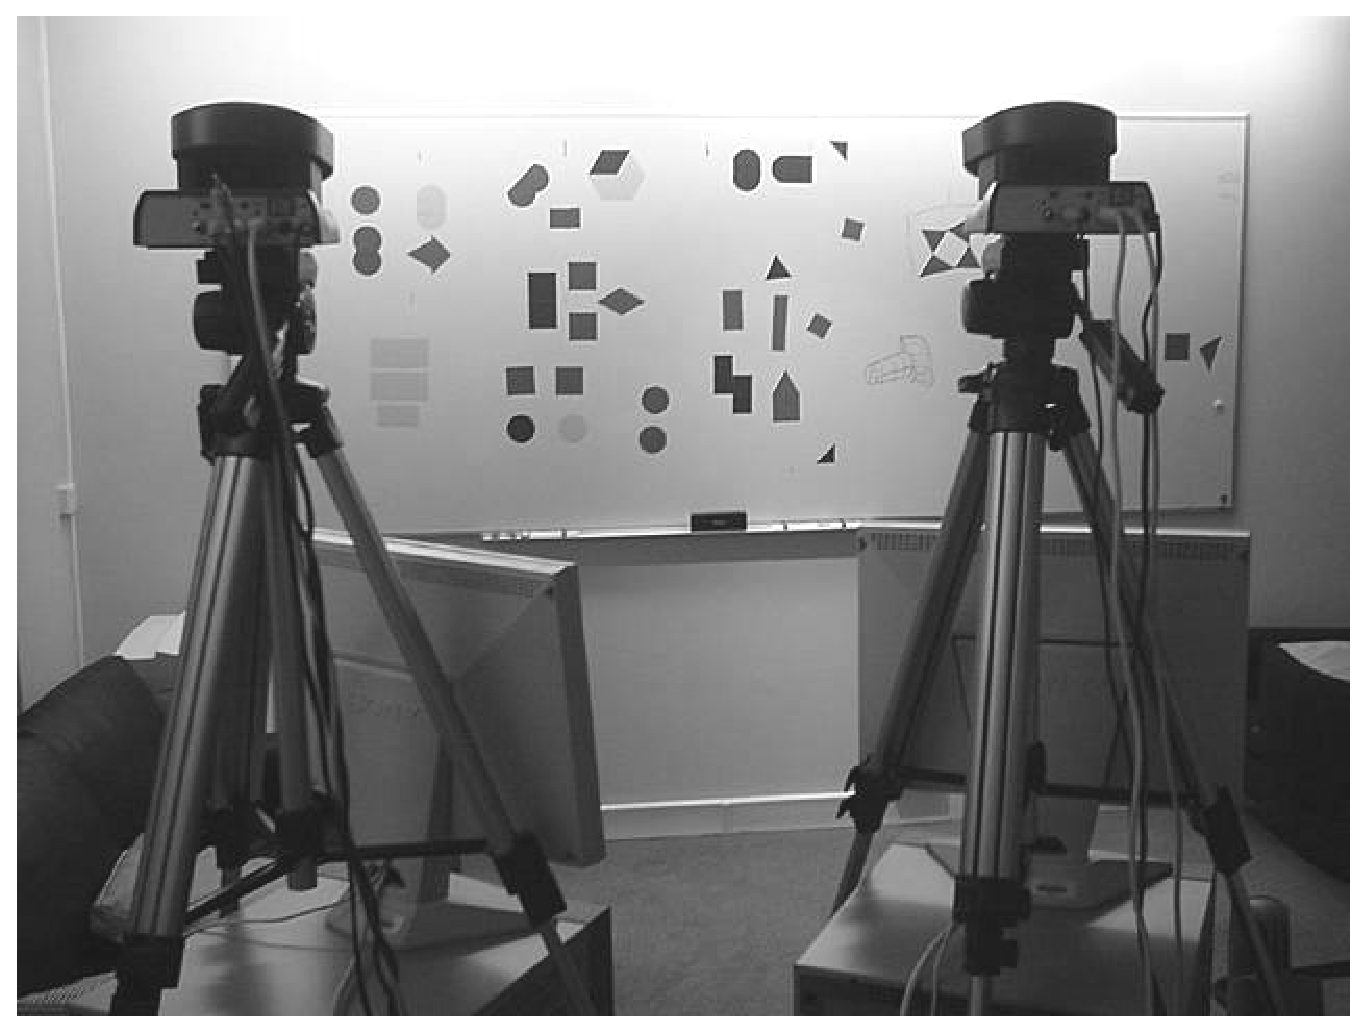
\includegraphics[width=12cm]{theory/th.eps}
\caption{The Talking Heads as it is installed at Sony CSL Paris.}
\label{f:theory:talkingheads}
\end{figure}

The Talking Heads consists of a couple of installations that are distributed around the world. Installations currently exist in Paris at the Sony CSL, in Brussels at the VUB AI Lab, in Amsterdam at the Intelligent Autonomous Systems laboratory of the University of Amsterdam. Temporal installations have been operational in Antwerp, Tokyo, Laussane, Cambridge, London and at another site in Paris. Agents can travel the world through the internet and embody themselves into a Talking Head. A Talking Head is a pan-tilt camera connected to a computer. The Talking Heads play language games with the cognitive capacities and memories that each agent has or has acquired. The language games are similar to the ones that are presented in the subsequent chapters. The main difference is that the Talking Heads do not move from their place, which the mobile robots do. The Talking Heads have cameras as their primary sensory apparatus and there are some slight differences in the cognitive capabilities as will become clear in the rest of this book.


\index{Talking Heads|)}
\index{Steels, Luc|)}
\index{Kaplan, Fr\'ed\'eric}
\index{AIBO}

All these experiments show similar results. Label-representation (or form-meaning) pairs can be grounded in sensorimotor control, for which (cultural) interactions, individual adaptation and self-organisation are the key mechanisms. A similar conclusion will be drawn at the end of this book. The results of the experiments on mobile robots will be compared with the Talking Heads as reported mainly in \citep{steels:2000}. Other findings based on the different variations of the model, which inspects the different influences of the model will be compared with the PhD thesis of Fr\'ed\'eric Kaplan of Sony CSL in Paris \citep{kaplan:2000}\footnote{Currently Fr\'ed\'eric Kaplan is working on human-machine interaction on the AIBO robot that looks like a dog and which has been developed by Sony CSL in Tokyo. Naturally, the AIBO learns language according to the same principles advocated by our labs.}.

\index{De Jong, Edwin}

A last set of experiments that will be brought to the reader's attention is the work done by Edwin de Jong of the VUB AI Lab. De Jong has done an interesting experiment in which he showed that the communication systems that emerged under the conditions by which language research is done in Paris and Brussels are indeed complex dynamical systems \citep{dejong:2000}. The communication systems of his own experiments all evolved towards an attractor and he showed empirically that the system was a complex dynamical system.

Using simulations, De Jong studied  the evolution of communication in experiments in which agents construct a communication system about {\em situation concepts} \citep{dejong:99b}. In his simulation, a population of agents were in some situation that required a response in the form of an action. I.e.  if one of the agents observed something (e.g. a predator), all the agents needed to go in some save state. De Jong investigated if the agents could benefit from communication, by allowing the agents to develop a shared lexicon that is grounded in this simulated world. The agents were given a mechanism to evaluate, based on their previous experiences, whether to trust on their observations or on some communicated signal. The signal is communicated by one of the agents that had observed something.

While doing so, the agents developed an ontology of situation concepts and a lexicon in basically the same way as in the work of Luc Steels. This means that the robots play discrimination games to build up the ontology and naming games to develop a language. A major difference is that the experiments are situated in a task oriented approach. The agents have to respond correctly to some situation. To do so, the agents can evaluate their success based on the appropriateness of their actions. As will be discussed in \chapref{ch:lg}, De Jong used a different method for categorisation, called the {\em adaptive subspace method} \citep{dejongvogt:1998}.

One interesting finding of De Jong was that it is not necessary that agents use feedback on the outcome of their linguistic interactions to construct a coherent lexicon, provided that the robots have access to the meaning of such an interaction and lateral inhibition was assured. Hence this confirms the findings of Mike \citet{oliphant:1998}. Questions about the feedback on language games are also issued in the field of human language acquisition.

\index{symbol grounding problem|)}

\index{child language acquisition|see{language!acquisition}}
\index{language!acquisition|(}
\section{Language Acquisition}\label{s:intro:acquisition}

Although children learn an existing language, lessons from the language acquisition field may help to understand how humans acquire symbols. This knowledge may in turn help to build a physically grounded symbol system. In the experiments presented in the forthcoming, the robots develop only a lexicon by producing and understanding one word utterances. In the literature of language acquisition, this period is called {\em early lexicon development}. Infants need to learn how words are associated with meanings. How do they do that?

In early lexicon development it is important to identify what cues an infant receives of the language it is learning. These cues not only focus on the linguistic information, but also on the extra-linguistic information. It is not hard to imagine that when no linguistic knowledge is available about a language, it seems impossible to learn such a language without extra-linguistic cues such as pointing or feedback about whether one understands a word correctly. (Psycho)linguists have not agreed upon what information is available to a child and to what extend.

The {\em poverty of the stimulus} argument led Chomsky to propose his linguistic theory. Although an adult language user can express an unlimited number of sentences, a language learner receives a limited amount of linguistic information to master the language. With this argument Chomsky concluded that linguistic structures must be innate. But perhaps there are other mechanisms that allow humans to learn language. Some might be learned and some might be innate.

\index{feedback}
\index{no negative feedback evidence}

A problem that occupies the nativist linguists is the so-called {\em no negative feedback evidence} (e.g. \citep{bowerman:1988}). The problem is that in the innate approach language can only be learned when both positive and negative feedback on language is available to a language learner. However, psychological research has shown that no negative feedback is provided by adult language users \citep{braine:1971}. Demetras and colleagues, however showed that there is more negative feedback provided than assumed \citep{demetrasetal:1986}. In addition, it is perhaps underestimated how much feedback a child can evaluate itself from its environment. Furthermore, feedback is thought to be an important principle in cognitive development, see e.g. \citep{clancey:1997}.

\index{joint attention}

One alternative for the feedback, which is assumed to be provided after the linguistic act, is the establishment of joint attention {\em prior} to the linguistic communication. Do children really receive such input? Early studies of Tomasello showed that children can learn better when joint attention is established, as long as this is done spontaneously by the child \citep{tomaselloetal:1986} cited in \citep{barrett:1995}. Explicit drawing of attention seemed to have a negative side effect. Although it has been assumed that pointing was a frequently used method to draw a child's attention, later studies have argued against such this assumption. Tomasello reported in a later studies that pointing is not necessary for learning language, {\em provided} there is explicit feedback \citep{tomasellobarton:1994}. 

In this article, Tomasello and Barton report on experiments where children learn novel words under two different conditions. In one condition, children do not receive extra-linguistic cues when the word-form is presented. There is a so-called {\em nonostensive} context. When at a later moment the corresponding referent is shown, a positive feedback is given if the child correctly relates the referent with given word-form. If the child relates the word-form to an incorrect referent, negative feedback is given. In the second condition, joint attention is established simultaneous with the presentation of the word-form. In this condition the child receives a so-called {\em ostensive} context. \citet{tomasellobarton:1994} showed in their experiments that children could equally well learn novel word-meaning relations in both condition.

Yet another strategy is proposed by Eve \citet{clark:1993}. She argues that children can fill in knowledge gaps when receiving novel language, provided the context was known. 


So, a lot of strategies appear to be available to a language learner, and there may be more. It is not unlikely that a combination of the available strategies is used; perhaps some more frequent than others. A natural question rises: Which strategies work and which do not? In this book experiments are presented that investigate both the role of feedback and joint attention.
\index{language!acquisition|)}


\section{Setting Up The Goals}\label{s:intro:goals}

This book presents the development and results of a series of experiments where two mobile robots develop a grounded lexicon. The experiments are based on language games that have first been implemented on mobile robots in \citep{steelsvogt:1997,vogt:1997}. The goal of the language games is to construct an ontology and lexicon about the objects the robots can detect in their environment.



The sensory equipment with which the robots detect their world is kept simple, namely sensors that can only detect light intensities. One of the goals was to develop the experiments without changing the simplicity of the robots very much and to keep the control architecture within the behaviour-based design. Luc \citet{steels:1996a} hypothesises three basic mechanisms for language evolution, which have been introduced above: individual adaptation, cultural evolution and self-organisation. 
\index{self-organisation}
\index{Steels, Luc}
\index{behaviour-based!architecture}

In a language game, robots produce a sensorimotor behaviour to perceive their environment. The environment consists of a set of light sources, which are distinguishable in height. The raw sensory data that results from this sensing is segmented, yielding a set of segments of which each segment relates to the detection of a light source. These segments can be described by features, which are categorised by the individual robots. The categorisation is processed by so-called {\em discrimination games} \citep{steels:1996b}. In this process the robots try to develop categories that discriminates one segment from another. The lexicon is formed based on an interaction and adaptation strategy modelled in what has been called {\em naming games} \citep{steels:1996a}. In a naming game one robot has the role of a speaker and the other robot has the role of the hearer. The speaker tries to name the categorisation (or meaning) of a segment it has chosen to be the topic. The hearer tries to identify the topic using both linguistic and extra-linguistic information when available.

\index{cultural evolution}
\index{Darwin, Charles}

The language game is adaptive in that the robots can adapt either their ontology or lexicon when they fail to categorise of name the topic. This way they may be successful in future games. In addition, the robots can adapt association strengths that they use to select elements of their ontology or lexicon. The selection principle is very much based on natural selection as proposed by Charles \citet{darwin:1968}, but the evolution is not  spread over generations of organisms, but over `generations' of language games. The principle is that the most effective elements are selected more and ineffective ones are selected less frequently, or even not at all. This way the most effective elements of the language are spread in the language community, thus leading to a {\em cultural evolution}.

\index{memes}
The idea of cultural evolution has best been described by Richard Dawkins in his book {\em The Selfish Gene} \citep{dawkins:1976}. In this book Dawkins proposes the notion of {\em memes}. Memes are elements that carry the notion of ideas, like the idea of a {\em wheel}. Like genes, memes are generated as varieties of previous ideas and possibly as complete new ideas. The memes are spread in the society by cultural interactions. The evolution of memes is similar to that of genetic evolution and good memes survive, whereas bad memes do not. However, the cultural evolution is much faster than biological evolution and several generations of memes can occur in a society within the lifetime of an organism. When changing the notion of memes into language elements, a cultural evolution of language arrives. The emergence of language through cultural evolution is based on the same principle as biological evolution, namely {\em self-organisation}.


Three main research questions are raised in this book:

\begin{enumerate}
\index{symbol grounding problem}
\item Can the symbol grounding problem be solved with these robots by constructing a lexicon through individual adaptation, (cultural) interaction and self-organisation? And if so, how is this accomplished?
\index{extra-linguistic information}
\item What are the important types of extra-linguistic information that agents should share when developing a coherent communication system?
\item What is the influence of the physical conditions and interaction of the robots on developing a grounded lexicon?
\end{enumerate}


The first question is an obvious one and can be answered with yes, but to a certain extend. As argued in \sectref{s:intro:semiotic}, the symbol grounding problem is solved when the robots are able to construct a semiotic sign of which the form is either arbitrary or conventionalised. Since the robots try to ground a shared lexicon, the form has to be conventionalised. Therefore the robots solve the symbol grounding problem when they successfully play a language game. I.e. when both robots are able to identify a symbol with the same form that stands for the same referent. 

Throughout the book the model that accomplishes the task is presented and revised to come up with two language game models that work best. Although the basics of the models, namely the discrimination- and naming game are very simple, the implementation on these simple robots has proven to be extremely difficult. Not all the designer's frustrations are made explicit in this book, but working with LEGO robots and ``home-made'' sensorimotor boards made life not easier. In order to concentrate on the grounding problem, some practical assumptions have been made leaving some unsolved technical problems. 

The two models that are proposed at the end of the experimental results show different interaction strategies that answer the second question. Both feedback and joint-attention are important types of extra-linguistic information necessary for agents to develop a lexicon, although not necessarily used simultaneously. How feedback and joint attention can be established is left as an open question. Technical limitations drove to leave this question open as one of the remaining frustrations. Some of these limitations are the same that introduced the assumptions that have been made. 

Although more difficult to show, the quality of physical interactions have an important influence on the robots' ability to ground a lexicon. When the robots are not well adapted to their environment (or vice versa) no meaningful lexicon can emerge. In addition, when the robots can co-ordinate their actions well to accomplish a certain (sub)task, they will be better in grounding a lexicon than when the co-ordination is weak.

\section{Contributions}

How does this book contribute to the field of artificial intelligence and cognitive science? The main contributions made in this book that there is an autonomous system that is grounded in the real world of which no parts of the ontology or lexicon is pre-defined. The categorisation is organised hierarchically by prototypical categories. In addition, the book investigates different types of extra-linguistic information that the robots can use to develop a shared lexicon. No single aspect is more or less unique. However, the combination of some aspects is.

Table \ref{t:intro:contrib} shows the contributions of research that is most relevant to this work. The table lists some aspects that the various researchers have contributed in their work. The aspects that are listed are thought to be most relevant to this work. Note that with Steels' work the Talking Heads experiments are meant. In the discussion at the end of this book, a more detailed comparison with the Talking Heads is made.

\begin{table}[t]
\begin{tabular}{>{\raggedright}p{3.5cm}cccccccc}
\lsptoprule
Aspect & B & C & D & O & R & S & V & Y\\\midrule
Grounded in real world & + & - & - & - & + & + & + & +\\\hline
Language pre-defined & + & + & - & - & $\cdot$ & - & - & +\\\hline
Meaning pre-defined & +/- & - & - & + & - & - & - & +\\\hline
Prototypical categories & - & - & - & $\cdot$ & + & - & + & -\\\hline
Hierarchical layering of categories & - & - & + & $\cdot$ & - & + & + & -\\\hline
Nr. of meanings given & +/- & - & - & + & - & - & - & +\\\hline
Nr. of forms given & + & + & - & + & $\cdot$ & - & - & +\\\hline
Nr. of agents & 2 & $\geq 2$ & $\geq 2$ & $\geq 2$ & 1 & $\geq 2$ & 2 & $\geq 2$\\\hline
Calibrated world & - & - & - & $\cdot$ & - & + & - & -\\\hline
Mobile agents & + & + & + & $\cdot$ & + & - & + & +\\\hline
Camera vision & - & $\cdot$ & $\cdot$ & $\cdot$ & - & + & - & -\\\hline
Autonomous & + & + & + & + & + & + & + & -\\\hline
Task oriented & + & + & + & - & - & - & - & +\\\hline
Extra-linguistic & - & - & + & + & $\cdot$ & - & + & -\\
\lspbottomrule
\end{tabular}
\caption{Various aspects investigated by different researchers. Each column of the table is reserved for a particular research. The related work in this table is from (the group of): B - Billard, C - Cangelosi, D - De Jong, O - Oliphant, R - Rosenstein, S - Steels, V - Vogt, Y - Yanco and Stein. The other 'symbols' in the table stand for '+' - yes, '-' - no and '$\cdot$' - not applicable.}
\label{t:intro:contrib}
\end{table}

\index{Billard, Aude}\index{Oliphant, Mike}\index{De Jong, Edwin}\index{Steels, Luc}

Of the related work, the work of \citep{cangelosiparisi:1998,dejong:2000,oliphant:1997} is not grounded in the real world. The work of Cangelosi et al. and De Jong is grounded only in simulations. This makes the grounding process relatively easy, because it avoids the problems that come about when categorising the real world. Oliphant does not ground meaning at all. The work of this book is grounded in the real world.

Some researchers, notably \citep{billard:1997a,cangelosiparisi:1998,yancostein}, pre-define the language. I.e. they define how a word-form relates to a behaviour or real world phenomenon. The pre-defined language in Billard and Hayes' experiments is only given to the teacher robot, the student robot has to learn the language. Although in the work of Yanco and Stein the robots learn the language, the researchers have pre-defined the language and they provide feedback whether the language is used successfully. \citet{rosenstein:1998a} do not model language yet. Hence the question if they pre-define the language is not applicable. In the work done at the VUB AI Lab no such relationships are given to the agents. This is also not given in the work of Mike \citet{oliphant:1997}. This means that the agents construct the language themselves. 

Meaning is pre-defined if the agents have some representation of the meaning pre-programmed. This is done in the work of \citep{billard:1997a,oliphant:1997,yancostein}. In the work of Billard and Hayes, the meaning is only given to the teacher robot. The student robot learns the representation of the meaning. Oliphant's agents only have abstract meanings that have no relation to the real world. In the work that is done in most of Steels' group the agents construct their own ontology of meanings.

Of the researchers that are compared with this work, only \citet{rosenstein:1998a} makes use of prototypes as a way of defining categories. All other work makes use of some other definition. This does not mean that the use of prototypes is uncommon in artificial intelligence, but it is uncommon in the 'grounding of language community'.

A hierarchical structuring of the categorisations is only done by the researchers of Steels' group, this book included. The advantage of hierarchical structuring of categories is that a distinction can be either more general or more specific.

Quite some researchers pre-define the number of meanings and/or forms that is, or should arise in the language \citep{billard:1997a,cangelosiparisi:1998,oliphant:1997,yancostein}. Naturally, language is not bound by the number of meanings and forms. Therefore, the number of meanings and forms is unbound in this book.

It may be useful if the position of the robot in relation to other robots and objects in their environment is known exactly. Especially for technical purposes, like pointing to an object. However, such information is not always known to the language users. In the Talking Heads experiment, the robots have calibrated knowledge about their own position (which is fixed) and the position of the other robot, and they can calculate the position of objects in their world. Such information is not available to the robots in this book. This is one of the main differences between the Talking Heads and the current experiments. Another difference with the Talking Heads is the use of camera vision, rather than low-level sensing. Still other differences are at the implementation of the model. These differences have been discussed above and will be discussed more in \chapref{ch:disc}.

Not all experiments deal with robots that are mobile in their environment. In particular the Talking Heads are not mobile, at least not in the sense that they can move freely in their environment. The Talking Heads can only go from physical head to physical head. The locations of these heads are fixed. 

Except the work of \citet{yancostein}, all experiments are autonomous, i.e. without the intervention of a human. Yanco and Stein give their robots feedback about the effect of their communication. This feedback is used to reinforce the connections between form and meaning. The system designed in this book is completely autonomous. The only intervention taken is to place the robots at a close distance rather than letting them find each other. This is done in order to speed up the experiments. In previous implementations, the robots did find each other themselves \citep{steelsvogt:1997}. There is no intervention at the grounding and learning level involved.

In most of the experiments mentioned, the agents have only one task: developing language. Some scientist argue that language should be developed in a task-oriented way, e.g. \citep{billard:1997a,cangelosiparisi:1998,dejong:2000,yancostein}. In particular, the task should have an ecological function. This seems natural and is probably true. However, in order to understand the mechanisms involved in lexicon development, it is useful to concentrate only on lexicon development. Besides, developing langauge is in some sense task-oriented.

As explained, one of the research goals is to investigate the importance of extra-linguistic information that guides the lexicon development. This has also been investigated by \citet{oliphant:1997} and \citet{dejong:2000}.

So, in many respects the research that is presented in this book is unique. It takes on many aspects of a grounded language experiment that is not shared by other experiments. The experiment that comes closest is the Talking Heads experiment. The results of the experiments from this book will therefore be compared in more detail at the end of this book.


\section{The Book's Outline}

The book is basically divided in three parts. In the first part, the model by which the experiments are developed is introduced. Part two presents experimental results. And the final part is reserved for discussions and conclusions.


Chapter \ref{ch:robots} introduces the experimental set-up. This includes the environment in which the robots behave and the technical set-up of the robots. This chapter explains the Process Description Language PDL in which the robots are programmed. PDL is for the purpose of these experiments extended from a behaviour-based architecture in a behaviour-based {\em cognitive} architecture. This is to enable better controllable planned behaviour. People not interested in the technical details of the robots may omit this chapter. For these people it is advisable to read \sectref{s:robots:envir} in which the environment is presented. In addition, the part on the white light sensors in \sectref{s:robots:sensors} is important to follow some of the discussions.

The language game model is introduced in \chapref{ch:lg}. It explains how the robots interact with each other and their environment. The interaction with their environment includes sensing the surroundings. The result of the sensing is pre-processed further to allow efficient categorisation. The discrimination game with which categorisation and ontological development is modelled is explained. After that, the naming game is presented, which models the naming part of the language game and the lexicon formation. The chapter ends with a presentation of how the discrimination game and the naming game are coupled to each other.


The experimental results are presented in chapters \ref{ch:basic}, \ref{ch:cat} and \ref{ch:opt}. Chapter \ref{ch:basic} first introduces the measures by which the results are monitored. The first experiment that is presented is called the {\em basic experiment}. A detailed analysis is made of what is going on during the experiment. As will become clear it still has a lot of discrepancies. These discrepancies are mostly identified in following chapters. 

The experiments presented in \chapref{ch:cat} are all variants of the basic experiment. In each only one parameter or strategy has been changed. The experiments investigate the impact from various strategies for categorisation, physical interaction, joint attention and feedback. In addition, the influence of a few parameters that control adaptation are investigated. Each set of experiments is followed by a brief discussion.

The final series experiments are presented in \chapref{ch:opt}. Two variants of the language games that have proven to be successful in previous chapters are investigated in more detail. Each of these experiments have a varying strategy of using extra-linguistic information and are additionally provided with parameter settings that appeared to yield the best results. The first experiment is the {\em guessing game} in which the hearer has to guess what light source the speaker tries to name, without previous knowledge about the topic. In the second experiment prior topic knowledge is provided by joint attention. No feedback on the outcome is provided in the second game, called the {\em observational game}.


Chapter \ref{ch:disc} discusses the experimental results and presents the conclusions. The discussion is centred on the research questions posed in the previous section. Additional discussions centre on the similarities and differences with related work, in particular with the work done by other members of the VUB AI Lab and Sony CSL Paris. Finally some possible future directions are given.
% LocalWords:  ALife




